\label{desenvolvimento_processamento}

Nesta seção é descrito o detalhamento da solução e finalização do módulo de Interface e Processamento, bem como mudanças que ocorreram e a descrição da integração final com todos os sub-módulos resultando na entrega do produto final previsto na Fase 04.

\subsection{Detalhamento do Módulo}

Nesta seção é resumida os principais pontos do módulo de Interface e Processamento, focando na Parte 3 (Projeto e Construção da Solução) de forma a sumarizar todo o trabalho que foi realizado até o momento da iniciação da Parte 4 (Integração).

\begin{itemize}
  \item A frente de Interface e Processamento é a frente de Engenharia de Software que terá as seguintes preocupações:
  \item Se comunicar e receber os dados da central de controle do sistema;
  \item Realizar o tratamento dos resultados recebidos;
  \item Realizar experimentos de vibração da mesa;
  \item Apresentá-los ao usuário na forma de indicadores condizentes ao objetivo do projeto;
\end{itemize}

Esses são os principais pontos que resumem todo o trabalho de Software em cima do sistema. E durante as iterações ocorridas na Parte 3 os seguintes tópicos abaixo foram realizados:

\begin{itemize}
  \item Refatoração do Protocolo de Comunicação;
  \item Mudança do banco de dados para o \textbf{MySQL};
  \item Pseudo-integração com simulador da central de controle do sistema;
  \item Refatoração do \textit{parser} para utilização do Banco de dados do servidor local, integrado a aplicação do servidor;
  \item Integração do \textit{REST} entre Aplicação Web e Aplicação do Servidor (\textbf{Raspberry});
  \item Mudança da linguagem do Protocolo de Comunicação na Aplicação \textit{Web} para \textbf{Python}. Embora testes executados isoladamente demonstraram um maior desempenho por parte da linguagem C, é válido ressaltar que a linguagem Python traz um ganho de produtividade, visto que já dispõe dos recursos necessários para serialização de dados. Se as rotinas de comunicação tivessem sido construídas com C, seria necessária uma etapa adicional para tratamento dos dados brutos, o que não é necessário com o Python, visto que o dado ao ser lido na porta serial já é armazenado em uma estrutura e serializado para envio do \textit{REST} para a Aplicação \textit{Web};
  \item Implementação do Algoritmo de Pausa do Experimento de acordo com a mudança de frequência entre \textbf{Jobs};
  \item Implementação dos gráficos na Aplicação Web;
  \item Implementação do novo Protocolo de Comunicação;
  \item Estudo e escolha do método de ajuste e processamento de curvas de acordo com resultados obtidos;
  \item Implementação do Método do Trapézio Acumulado para processamento da curva;
  \item Implementação de Sincronização de \textbf{Threads} para escrita e leitura de dados da porta serial;
  \item Implementação do Sistema de \textbf{Jobs} e Ensaio para o controle da Bancada em alto nível.
\end{itemize}

A parte 3 foi focada em deixar o módulo o mais independente possível e pronto para ser integrado (com uso de simulações) com a parte de Eletroeletrônica. Com utilização de simulações e manipulações de \textbf{bytes} até ao alto nível de controle do usuário, Software desenvolveu duas aplicações separadas responsáveis pela manipulação de dados e entregar e controle dos dados em nível de usuário.

Com o fim da parte 3, a frente de interface e processamento terminou de produzir o módulo funcional, pronto para ser integrado ao sistema como um todo, principalmente com Eletroeletrônica pelo protocolo previamente definido, de acordo com a imagem abaixo.

\begin{figure}[H]
  \centering
  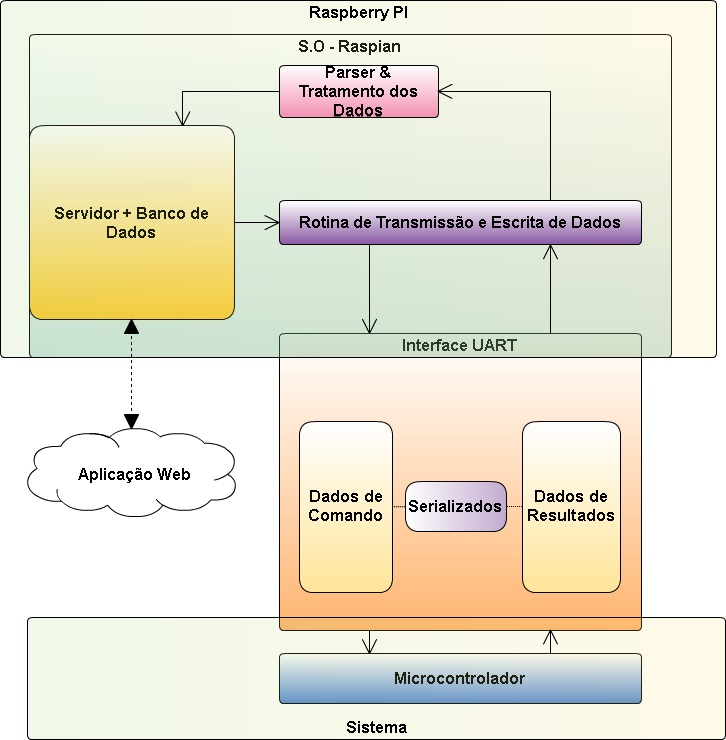
\includegraphics[keepaspectratio=true,scale=0.7]{figuras/nova_arquitetura.png}
  \label{fig:nova_arquitetura}
  \caption{Arquitetura Entregue do Módulo - Fonte: Autores}
\end{figure}

%%%%%%%%%% SUMARIZAR TODO O TRABALHO QUE FOI FEITO ATÉ AGORA PARA ENTREGA O SUBMÓDULO %%%%%%%%%%%%%%

\subsection{Detalhamento da Integração Final}

\subsection{Disponibilização da \textit{raspberry pi} como servidor}

Com uma \textit{raspberry Pi} é possível disponibilizar serviços em rede, estabelecer esquemas de computação em nuvem, configurar servidor FTP (\textit{File Transfer Protocol}) etc. Portanto, faz-se necessário configurá-la para que possa ser acessível de qualquer ponto da internet. No caso deste projeto, foi construída uma aplicação \textit{REST} que, por sua vez, será hospedada em uma \textit{raspberry pi}.

A figura a seguir ilustra de maneira esquemática a comunicação da \textit{Raspberry Pi} com a rede mundial, ou seja, a internet.

\begin{figure}[H]
\centering
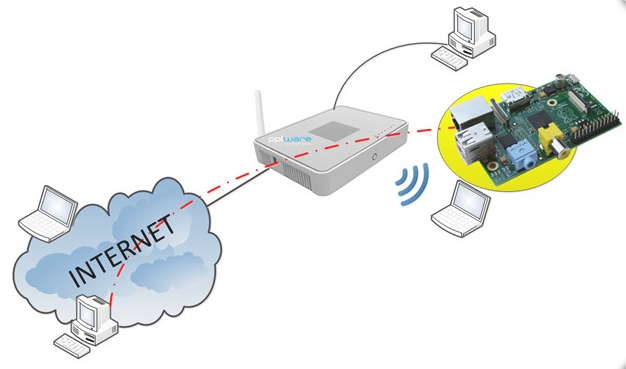
\includegraphics[keepaspectratio=true,scale=0.52]{figuras/raspberryeinternet.png}
\label{fig:raspberry_internet}
\caption{\textit{Raspberry Pi} e comunicação com a internet - Fonte: pplware}
\end{figure}

Primeiramente, é necessário criar uma conta em algum serviço que promova a identificação do dispositivo por meio de um nome, em outras palavras, configura-se um DNS (\textit{Domain Name System}) dinâmico. Um serviço existente hoje que oferece esse mapeamento é o no-ip (www.no-ip.org). A figura a seguir ilustra a página inicial do site.

\begin{figure}[H]
\centering
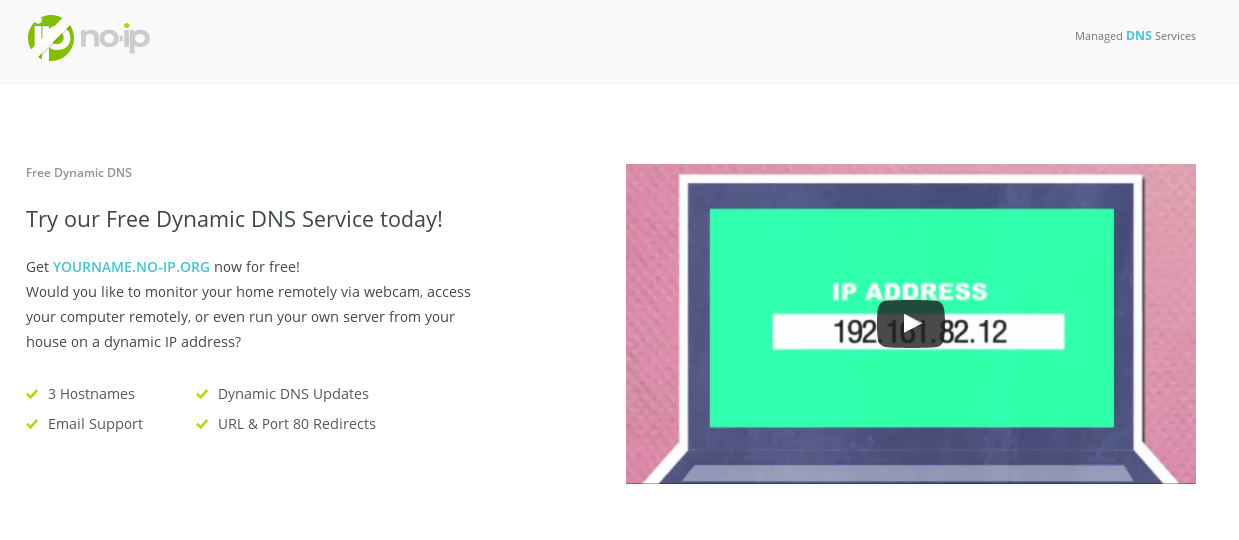
\includegraphics[keepaspectratio=true,scale=0.35]{figuras/sitenoip.png}
\label{fig:site_no_ip}
\caption{Página inicial do site no-ip}
\end{figure}

Com o serviço no-ip, o utilizador passa a identificar a \textit{raspberrypi} por um nome, a partir de qualquer lugar. A configuração permite usar sempre o mesmo nome para identificar o dispositivo, independentemente se o endereço IP (\textit{Internet Protocol}) público tiver sido alterado. É válido ressaltar que o serviço no-ip disponibiliza agentes que, por sua vez, são instalados do lado do cliente e assim, informam e atualizam os dados relativos ao endereço IP público. O agente caracteriza-se como um pequeno \textit{software} instalado na \textit{raspberry pi} e fornecido pelo serviço no-ip.

Prosseguindo com a configuração, faz-se necessário a configuração do mecanismo \textit{Port Forwarding}. Dessa maneira, todas as requisições que chegam ao roteador são redirecionadas para a porta configurada na \textit{raspberry pi}, por exemplo a porta 8080.

Ao final de todo este processo, será possível acessar a \textit{raspberry pi} de qualquer local, possibilitando a hospedagem de serviços.

\subsection{Aplicação Web}

Da aplicação Web, a sua integração se fez em garantir a integridade do dado que chega pelo protocolo de comunicação entre a central de comando até ao usuário final.

A integração que foi desenvolvida entre esses dois subsistemas que compõem o módulo de interface/processamento e deste módulo com o sistema todo, funciona da seguinte forma, entre a aplicação Web/ aplicação do Servidor e a Comunicação via Serial:

\begin{enumerate}
 \item O usuário cadastrado autentica-se no sistema (caso o usuário não seja cadastrado basta ele se cadastrar);
 \item O usuário monta um ensaio com seus respectivos \textit{jobs};
 \item O usuário confere os sensores ativos identificados pelo sistema e inicia o experimento;
    \subitem O usuário tem a possibilidade de atualizar os sensores ativos, caso perceba erro na leitura dos sensores;
    \subitem Quando o usuário solicita a identificação dos sensores ativos, a aplicação web envia uma requisição de identificação dos sensores ativos ao Servidor de Controle, seguindo o protocolo definido.
 \item A aplicação web envia uma requisição ao Servidor de Controle informando os dados dos \textit{jobs} e sinalizando que o experimento começou;
       \subitem A cada novo \textit{job} que deve começar (mudança de frequência da mesa) a aplicação web envia uma requisição de solicitação de alteração de frequência da mesa, seguindo o protocolo definido.
 \item O Servidor de Controle, então, envia uma mensagem ao sistema de controle (via rotinas de comunicação, informando o início do experimento e a frequência desejada (frequência do \textit{job} corrente) e inicia uma \textit{thread} para a coleta dos dados lidos dos sensores;
 \item Quando o último \textit{job} chegar ao fim, a aplicação web envia uma requisição ao Servidor de Controle informando que o ensaio acabou, o que significa que o sistema de controle não precisa mais coletar dados dos sensores;
 \item Quando o Servidor de Controle recebe essa requisição, este envia uma mensagem ao sistema de controle (via rotinas de comunicação) informando a parada da coleta dos dados dos sensores, seguindo o protocolo definido;
 \item A aplicação web informa ao usuário que está aguardando o término da coleta e processamento dos dados enquanto o Servidor de Controle coleta o restante dos dados dos sensores e a aplicação web processa os dados coletados;
 \item Quando todos os dados amostrados forem coletados, o Servidor de Controle repassa esses dados para a aplicação web e destes serão derivados os outros dados necessários para a aplicação, seguindo o método do trapézio acumulado. O processamento dos dados aqui mencionado se refere aos cálculos da frequência, velocidade e amplitude a partir da aceleração fornecida pelos sensores;
 \item Com todos os dados calculados, a aplicação web monta os gráficos e apresenta os resultados do ensaio ao usuário.
\end{enumerate}

Por fim, todas essas funcionalidades enumeradas acima foram desenvolvidas, contando com os adicionais como, gráficos por Job e o sistema de pausas. O sistema conta também com um sistema de tratamento de exceções para que nenhuma seja exibida a nível de usuário.

O processamento foi realizado utilizando a biblioteca do Python Scipy, uma biblioteca matemática para diversos calculos com base no próprio C. Com isso foi utilizado para realizar o processamento dos dados utilizando trapézio acumulado para se obter a curva aproximada dos pontos.

\subsection{Aplicação Server - Raspberry}

A aplicação de servidor da Raspberry teve uma mudança signifcativa, que foi o abandono do Banco de Dados, e a utilização direta de um JSON serializado para diminuição do tempo de envio dos dados, pois esses dados irão subir diretamente via REST para a camada de aplicação e serão processados de acordo com os respectivos dados a serem obtidos. Serão 1200 dados por segundo de 6 sensores pré-estabelecido, logo a taxa de transmissão de dados é muito alta, foi tomado todo o cuidado para que esse dado chegasse com sua integridade na camada de aplicação do usuário.

A integração frente Eletroeletrônica e Interface/Processamente está formalizada com o Protocolo funcional que permite o envio e o recebimento de dados do sistema de baixo nível para alto nível. Com o protocolo implementado na frente de Eletroeletrônica, a frente de Interface/Processamento conseguiu consolidar o envio e o recebimento de dados via portas UART (Tx/Rx) comunicação Serial.

O sistema está todo previamente testado e pronto garantindo a integridade do módulo como um todo, também integrado ao produto, assim, controlando o motor de acordo com as especificações dos Jobs de um Ensaio total, e recebendo os dados dos sensores conforme combinado, apresentando-os na forma de gráficos.

%%%%%%%%%% REALIZAR DETALHAMENTO DO TRABALHO DE INTEGRAÇÃO FINAL %%%%%%%%%%%%%%%

% Nesta seção é descrito o detalhamento da solução do módulo de interface/processamento, resultante das duas primeiras fases,
% e o seu projeto e construção, resultante da Fase 03.
% Além disso, a visão da solução e da arquitetura estão documentadas nos Apêndices \ref{documento_visao} e \ref{documento_arquitetura}, respectivamente.

% \subsection{Detalhamento da Solução} \label{software:detalhamento_solucao}

% A solução completa definida nas Fases 01 e 02 pode ser vista no \href{https://drive.google.com/file/d/0B5InkGKx6O-MR1B3eVYzZFpjQ3c/view?usp=sharing}{Relatório 1}.

% A Figura \ref{fig:arquitetura_solucao} apresenta a solução proposta como um todo e nela podemos destacar a atuação da
% frente de interface/processamento nos seguintes subsistemas de software:

% \begin{itemize}
%  \item \textbf{Interface de comunicação entre o usuário e a bancada, realizada por meio da aplicação web;}
%       \subitem Na aplicação web o usuário poderá controlar a bancada, iniciando um ensaio com os quesitos definido por ele,
% 	       e visualizar os resultados do ensaio por meio de gráficos.
%  \item \textbf{Servidor de Controle para intermediar a comunicação da aplicação web com o sistema de controle eletrônico, hospedado na \textit{Raspberry}.}
%       \subitem Este servidor provê serviços RESTFul (API REST) como a interface de comunicação para a aplicação web. Neste servidor estão as
% 	       rotinas de comunicação com o sistema de controle eletrônico, que realizam a inserção de dados de comando e recupera os dados
% 	       dos sensores via comunicação serial.
% \end{itemize}

% Nas próximas subseções são detalhados os dois subsistemas propostos como solução para o módulo de interface de processamento.


% \subsection{Projeto e Construção}

%   Nesta subseção é apresentado o projeto e construção dos subsistemas propostos na Subseção \ref{software:detalhamento_solucao},
%   bem como as mudanças realizadas no que foi proposto.

% \subsubsection{\textbf{Interface de comunicação com o usuário - Aplicação Web}} \label{software:app_web}

%     Como  apresentado no \href{https://drive.google.com/file/d/0B5InkGKx6O-MR1B3eVYzZFpjQ3c/view?usp=sharing}{Relatório 1},
%     a aplicação web servirá para o usuário controlar a bancada e visualizar os resultados dos ensaios, contando com os seguintes requisitos
%     funcionais (conforme \textit{backlog} apresentado no \href{https://drive.google.com/file/d/0B5InkGKx6O-MR1B3eVYzZFpjQ3c/view?usp=sharing}{Relatório 1})
%     para atender as necessidades do usuário (vide Apêndice \ref{documento_visao} para as necessidades do usuário):

%     \begin{itemize}
%       \item \textbf{Cadastro de usuários;}
% 	 \subitem Os usuários da bancada (alunos, professores e técnicos) devem ser cadastrados no sistema para utilizar a bancada.
%       \item \textbf{Acesso ao sistema;}
% 	 \subitem Os usuários cadastrados devem ter acesso ao sistema para realizar ensaios.
%       \item \textbf{Início do ensaio;}
% 	 \subitem Deve ser possível a criação de um ensaio específico pelo usuário, informando a frequência e tempo de ensaio desejados.
%       \item \textbf{Visualização dos ensaios realizados;}
% 	 \subitem Os ensaios de um usuário devem ser mantidos no sistema, para que o usuário possa visualizar os resultados de um ensaio
% 		  já realizado quando quiser;
%       \item \textbf{Visualização dos resultados do ensaio;}
% 	 \subitem Os resultados do ensaio realizado deve ser apresentado em formas de gráficos para facilitar a interpretação dos resultados.
%     \end{itemize}

%     Para o requisito "Início do ensaio" o usuário necessita poder criar um ensaio com diferentes frequências a serem testadas no mesmo ensaio.
%     Para implementar este requisito foi realizada um abstração do ensaio como um conjunto de \textit{jobs}.
%     Um \textit{job} é uma parte do ensaio com uma frequência e tempo fixo. Exemplificando, caso o usuário queira um ensaio que começa com uma
%     frequência de 50Hz por 10s e depois mude para 80Hz e permaneça por mais 15s, basta criar um ensaio com dois \textit{jobs}, onde o primeiro
%     \textit{job} teria frequência igual a 50Hz e tempo de 10s e o segundo teria frequência igual a 80Hz e tempo de 15s.

%     Com o intuito de visualizar a solução Web foi desenhado um protótipo de alta fidelidade da aplicação Web.
%     As telas podem ser vistas no \href{https://drive.google.com/file/d/0B5InkGKx6O-MR1B3eVYzZFpjQ3c/view?usp=sharing}{Relatório 1}.

%     Como definido no \href{https://drive.google.com/file/d/0B5InkGKx6O-MR1B3eVYzZFpjQ3c/view?usp=sharing}{Relatório 1},
%     a aplicação web foi desenvolvida utilizando o \textit{framework} Django (em linguagem Python) de acordo com as justificativas
%     apresentadas também no Relatório 1.

% \subsubsection{\textbf{Interface de comunicação com o sistema de controle - Servidor de Controle}}

%    Esta subseção apresenta o projeto e construção do servidor RESTFul que será hospedado na \textit{Raspberry} para intermediar a comunicação
%    com o sistema de controle. Este servidor é chamado aqui de Servidor de Controle.

% \subsubsubsection*{\textbf{Mudanças - Aspectos gerais}}

% Ao final do primeiro ponto de controle, a frente de interface/processamento, em suma, havia estabelecido os seguintes requisitos não-funcionais para o \textbf{software}:

% \begin{itemize}
%     \item Aplicação \textit{Web} para uso por parte do usuário, sendo esta desenvolvida com o \textit{framework} Django (que utiliza linguagem de programação \textit{Python}) juntamente com o SGBD (Sistema Gerenciador de Banco de Dados) \textit{MySQL}.
%     \item Aplicação \textit{REST} para recebimento de comandos e fornecimento de dados para a Aplicação \textit{Web}, sendo esta desenvolvida com o Django \textit{REST} \textit{Framework} juntamente com a base de dados \textit{SQLite}.
%     \item Rotinas de comunicação em linguagem C para escrita e leitura de dados na porta serial existente na \textit{Raspberry}.
% \end{itemize}


% Durante a execução do projeto, constatou-se que não haveria mais necessidade de uso da linguagem C, aspecto que será melhor detalhado na
% próxima subseção, sobre as mudanças no projeto das rotinas de comunicações.
% Outro aspecto alterado foi a base de dados utilizada pelo \textit{REST}, optando-se pelo uso do \textit{MySQL} ao invés do \textit{SQLite}.

% O SGBD \textit{MySQL} foi também adotado para a aplicação \textit{REST} pelos seguintes motivos:

% \begin{itemize}
%   \item É mais performático que o \textit{SQLite}.
%   \item Não há travamentos da base de dados devido às operações, o que possibilita a concorrência no uso do banco de dados.
%   \item Favorece a escalabilidade da solução.
% \end{itemize}

% \subsubsubsection*{\textbf{Arquitetura das Rotinas de Comunicação e Parser}} \label{software:rotinas}

% Para realização das rotinas de comunicação e parser, a equipe de software contou com um simulador. O simulador, construído pela frente de eletroeletrônica,
% consiste em um \textit{Arduino} que simula o comportamento da entrada e saída de dados que o sistema da \textit{Raspberry} terá de comunicar. Com isso
% então, foi possível realizar o desenvolvimento das rotinas de comunicação em \textit{Python}, bem como iniciar também o \textit{Parser}.

% O \textit{Parser} dos dados foi construído baseado na \textit{String} de resposta definida no protocolo de comunicação e em seguida essa \textit{String}
% é tratada para que seja guardada no banco de dados da aplicação local.
% O primeiro passo consiste realizar o tratamento dos dados em uma lista de forma a averiguar se os dados estão corretos de acordo com o padrão de
% resposta definido no protocolo de comunicação. O próximo passo então é inserir os dados da lista no banco de dados.

% % Com relação às rotinas de entrada e saída de dados, foi utilizado o \textit{Arduino} para fins de teste de comunicação. A frente de eletroeletrônica
% % desenvolveu uma rotina que é executada no \textit{Arduino} que conseguia simular a entrada e saída de dados com o comportamento similar ao esperado.

% Com relação às rotinas de entrada e saída de dados foi utilizada a biblioteca serial padrão no \textit{Python},
% foi possível construir métodos abstraindo o controle da comunicação serial em baixo
% nível para um alto nível e conectá-los às rotinas que guardarão os dados, no caso o \textit{Parser}.

% Para comunicação com o sistema de controle, foi desenvolvida uma classe que abstrai os principais métodos da
% biblioteca serial padrão do \textit{Python}, a classe "\textit{PiSerial}".
% Com essa biblioteca foi possível inicializar os valores como \textit{Baudrate} (Taxa de transmissão),
% \textit{Timeout} e a porta serial de entrada e saída dos dados. A classe também conta com um método simples
% que acumula os resultados de leitura da porta serial em uma grande lista que será utilizada pelo \textit{Parser}
% para o tratamento dos dados resultantes para que eles possam ser guardados no banco de
% dados. A classe também conta com um tratamento de exceções para evitar que as exceções subam a nível de usuário.

% A classe "\textit{Routine}" foi criada para comportar as rotinas disponíveis no sistema.
% Nesta classe são definidas as rotinas de leitura de dados resultantes, dos sensores ativos e da escrita de controle do sistema.
% Esta classe utiliza a classe  "\textit{PiSerial}" para realizar o gerenciamento da porta serial.

% Por fim, uma classe de faixada foi criada para receber as requisições de acesso à porta serial por parte dos serviços RESTFul
% do Servidor de Controle, a classe "\textit{SerialFacade}". Esta classe se comunica com a classe "\textit{Routine}" para chamar as
% respectivas rotinas necessárias.

% A integração entre eletroeletrônica e software vem com as rotinas que irão se comunicar com a malha fechada de controle do sistema e com a
% \textit{Raspberry} da aplicação, responsáveis por armazenar os resultados e repassá-los para a aplicação web.
% Na Figura \ref{fig:uml_routines_parser} é apresentado o diagrama de classes das rotinas de comunicação em integração
% com o Servidor de Controle.

% \begin{figure}[H]
% \centering
% 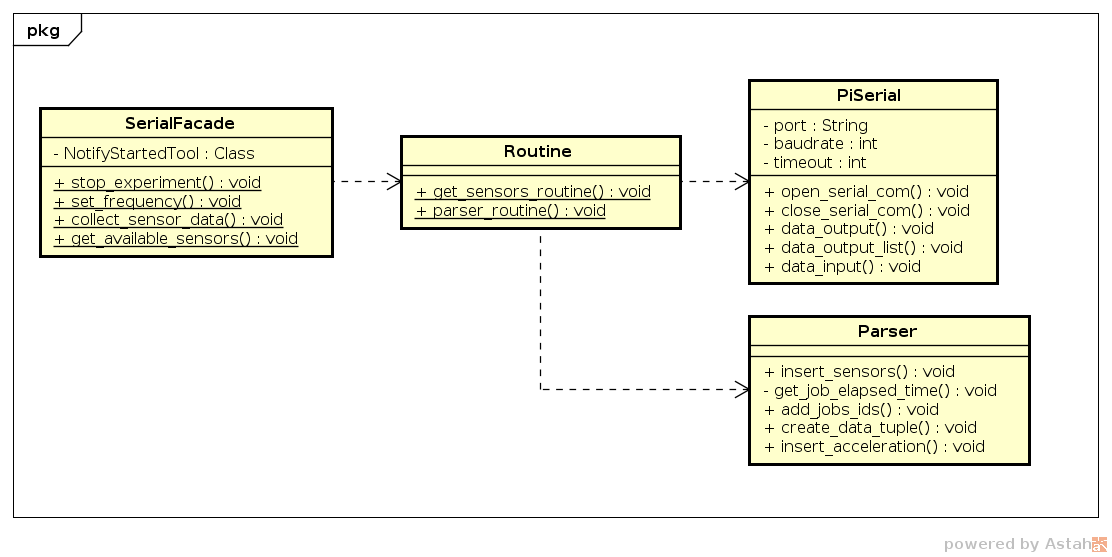
\includegraphics[keepaspectratio=true,scale=0.65]{figuras/diagrama_classe_rotinas.png}
% \label{fig:uml_routines_parser}
% \caption{Diagrama de Classes das Rotinas de Comunicação e Parser, integrados ao \textit{Django} - Fonte: Autor}
% \end{figure}


% \subsubsubsection*{\textbf{Mudanças - Rotinas de Comunicação}}

% A camada de software na aplicação Web foi desenvolvida em \textit{Python}, bem como a camada de servidor de comunicação com a aplicação na
% \textit{Raspberry}. Como foi relatado, os membros do grupo naquele momento haviam chegado ao consenso de utilizar a linguagem C para integrar
% com \textit{Python}, que seria utilizado nas rotinas de comunicação entre \textit{Raspberry} e os microcontroladores da aplicação de baixo nível.

% Durante o desenvolvimento das rotinas de comunicação, percebeu-se que não havia necessidade de que as mesmas fossem desenvolvidas
% usando tal linguagem, considerando que a linguagem C é uma linguagem de baixo nível normalmente utilizada para ter um maior controle sobre o
% hardware, o que não é o caso do projeto. Levando em consideração este fato, foi levantada a hipótese de utilização do módulo de comunicação serial que o próprio
% \textit{Python} oferece, e para isso foi realizado uma lista de prós e contras acerca da linguagem no desenvolvimento das rotinas de comunicação.

% Utilizando a linguagem C para o desenvolvimento das rotinas de comunicação possui as seguintes vantagens:

% \begin{itemize}
%     \item A linguagem C é uma linguagem de baixo nível, ou seja, oferece um maior controle do hardware, e fornece a possibilidade de manipulações com \textit{bytes} em uma maior flexibilidade do que com as demais linguagens, exceto a linguagem \textit{ASSEMBLY}.
%     \item Com a linguagem C é possível desenvolver o sistema de forma a se proteger contra falhas críticas, impedindo de repassar erros de baixo nível para a camada de alto nível.
%     \item A linguagem C realiza processamentos mais velozes em comparação com as outras linguagens como \textit{Python}, dentre outras, se tornando uma excelente ferramenta para manipulação de \textit{bytes}.
% \end{itemize}

% Desvantagens da utilização da linguagem C para o desenvolvimento das rotinas de comunicação:

% \begin{itemize}
%     \item Por ser uma linguagem de baixo nível com uma alta tipagem, o trabalho de desenvolver uma rotina de comunicação serial usando recursos da camada de hardware se tornam bastante complexos.
%     \item Na arquitetura proposta no primeiro ponto de controle, as rotinas de escrita e leitura de dados funcionariam da seguinte maneira: a escrita iria ler um arquivo, em seguida iria apagá-lo e então, enviaria este dado para o sistema de controle; no sistema de leitura, seria aberta a porta seria para leitura dos \textit{bytes}, que seriam decodificados e transcritos num arquivo para serem lidos por uma rotina \textit{Python} para escrever no banco de dados. Ou seja, a integração possui uma alta complexidade.
%     \item Apesar da linguagem C ser mais rápida que \textit{Python}, não existe necessidade das rotinas serem desenvolvidas em tal linguagem, pois a diferença de velocidade de escrita e leitura para comunicação serial é bem mínima levando em consideração ao que \textit{Python} também faz.
% \end{itemize}

% Vantagens em utilizar \textit{Python} para o desenvolvimento das rotinas de comunicação:

% \begin{itemize}
%     \item Python possui uma baixa tipagem.
%     \item Possui uma biblioteca de comunicação serial que realiza a abstração do jeito que o desenvolvedor quiser (seja controlar em baixo nível, ou em alto nível com uma abstração do controle).
%     \item Fácil integração com \textit{RESTful} do \textit{Django} que é realizado em \textit{Python}.
%     \item Elimina necessidade de escrever e ler em arquivos, pois os métodos podem ser carregados pelo \textit{REST} diretamente, assim o \textit{REST} terá o controle total da comunicação.
%     \item Não existe necessidade de manipular leitura e escrita de bytes, devida a abstração da biblioteca.
%     \item \textit{Python} é uma linguagem melhor para manipulação de dados, e permitirá a escrita dos dados recebidos diretamente no banco de dados do servidor da \textit{Raspberry}, que a aplicação irá utilizar.
% \end{itemize}

% Desvantagens da linguagem \textit{Python} para o desenvolvimento das rotinas de comunicação:

% \begin{itemize}
%     \item \textit{Python} é uma linguagem interpretada e mais lenta em comparação à linguagem C.
%     \item Não fornece um controle maior em comparação às linguagens de baixo nível.
% \end{itemize}

% Com a nova mudança então, a única linguagem de programação que está sendo utilizada neste projeto é a linguagem \textit{Python}, e em virtude
% desta mudança, a arquitetura mudou um pouco agora, sendo nesse novo estilo.

% \begin{figure}[H]
% \centering
% 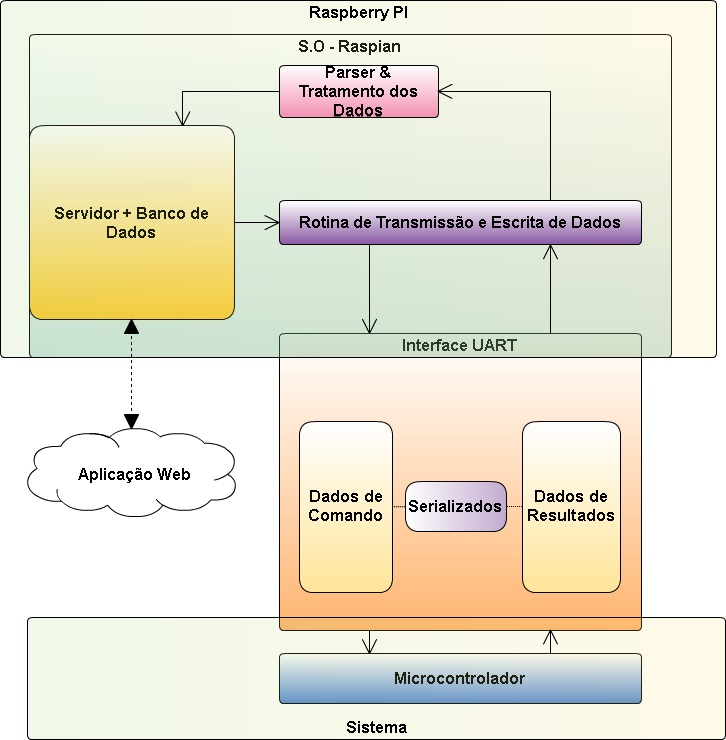
\includegraphics[keepaspectratio=true,scale=0.7]{figuras/nova_arquitetura.png}
% \label{fig:nova_arquitetura}
% \caption{Nova arquitetura com a mudança da linguagem implementada - Fonte: Autor}
% \end{figure}

% \subsubsection*{\textbf{Processamento dos Dados}} \label{software:processamento}

% Como mencionado, o processamento dos dados se refere ao cálculo da frequência, velocidade e amplitude a partir dos dados de aceleração
% coletados dos sensores. Como os dados que se tem são coordenadas de aceleração por tempo, é preciso recorrer a integração numérica para
% cálcular esses dados, pois a velocidade (v(t)) é a integral da aceleração (a(t)) e o deslocamento (s(t)) é a integral da velocidade, como
% ilustram as fórmulas abaixo. A curva do deslocamento, neste caso, representa a amplitude (A) ao longo do tempo, pois o deslocamento calculado
% da mesa, a partir dos dados dos sensores, representa o quanto a mesa subiu ou desceu (pois a mesa se move apenas no eixo Y).

% $$ v(t) = \int_{}^{} a(t) dt$$
% $$ A(t) = s(t) = \int_{}^{} v(t) dt$$

% \subsubsubsection*{\textbf{Métodos numéricos analisados}}

% A integral é uma das mais importantes ferramentas matemáticas e que aparece com frequência na solução de problemas e no cálculo de grandezas
% na engenharia e na ciência \cite{metodos_numericos}.

% Na engenharia, há situações que envolvem dados experimentais ou de teste, nos quais uma grandeza física a ser determinada pode ser expressa
% como a integral de outras grandezas medidas. Assim, é válido ressaltar que o integrando pode ser uma função analítica ou um conjunto de pontos
% discretos (dados tabulados).

% Quando se tem um integrando expresso de forma que a integral pode ser facilmente calculada, pode-se obter analiticamente o valor da integral
% definida. A integração numérica faz-se necessária quando a integração analítica é difícil, ou mesmo impossível, e quando o integrando é fornecido
% como um conjunto discreto de pontos \cite{metodos_numericos}.

% Este é o caso da Bancada de Vibrações Mecânicas que está sendo construída neste projeto. Os dados que se tem são o retorno da leitura dos sensores
% e assim, o integrando é fornecido como um conjunto de pontos.

% A análise numérica de uma integral caracteriza-se por estimar o número correspondente à integral de uma função entre os limites [a, b].
% Caso seja utilizado apenas os pontos finais do intervalo, pode ser que o resultado fornecido não seja suficientemente preciso, especialmente se
% o intervalo for significativamente grande ou se o integrando variar significativamente ao longo do intervalo. Dessa maneira, uma maior precisão
% pode ser obtida com o uso de um método composto, no qual o intervalo [a, b] é dividido em subintervalos menores. Assim, calcula-se a integral ao
% longo de cada subintervalo e os resultados são somados para fornecer a integral completa.

% É importante ressaltar que existem vários métodos disponíveis para o cálculo numérico de integrais. Esses métodos podem ser divididos em abertos
% e fechados. Os métodos de integração fechados consideram os pontos finais do intervalo e o integrando propriamente dito na fórmula que estima o
% valor da integral. Já nos métodos de integração abertos, o intervalo de integração se estende além do limite especificado pelos pontos finais
% \cite{metodos_numericos}.

% Devido à variedade de métodos, os principais foram analisados e verificou-se sua aplicação no âmbito do projeto. Os métodos considerados foram:
% Trapezoidal Composto, Métodos de Simpson e Quadratura de Gauss.

% No {\textbf{Método Trapezoidal Composto}} a integral, ao longo do intervalo [a, b], pode ser avaliada de forma mais precisa com a subdivisão do
% intervalo, a avaliação da integral em cada um dos subintervalos e a soma dos resultados. A imagem a seguir ilustra a expansão genérica para a
% integração numérica por trapézios.

% \begin{figure}[H]
% \centering
% 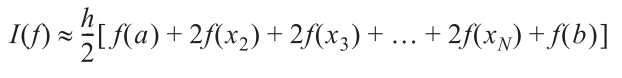
\includegraphics[keepaspectratio=true,scale=0.52]	{figuras/metodo_trapezoidal.png}
% \label{fig:metodo_trapezoidal}
% \caption{Integração numérica por Trapézios Acumulados - Fonte: \citeonline{metodos_numericos}}
% \end{figure}

% É importante notar que a fórmula do método trapezoidal composto se aplica precisamente para os casos onde os subintervalos têm uma largura h
% idêntica. Outro aspecto interessante no uso desse método é que a precisão da resposta pode melhorar a partir da utilização de mais subintervalos.

% O método trapezoidal aproxima o integrando por uma linha reta. De fato, seria melhor a aproximação por meio da representação do integrando
% como uma função não-linear e de fácil integração.

% Há um grupo de métodos dotados desta característica, denominados \textbf{Métodos de Simpson}, utilizando polinômios quadráticos (método de
% Simpson 1/3) e polinômios cúbicos, no caso do método de Simpson 3/8.

% Os métodos de Simpson possuem restrições mais severas para uso. No caso do método de Simpson 1/3 composto, os subintervalos devem ser
% igualmente espaçados e o número de subintervalos no intervalo [a, b] deve ser um número necessariamente par. Com relação ao método de Simpson
% 3/8 composto, além do espaçamento igual na identificação dos subintervalos, tem-se que o número de subintervalos no intervalo [a, b] deve ser
% divisível por 3.

% Por fim, na \textbf{Quadratura de Gauss}, a integral também é avaliada utilizando a soma ponderada dos valores da função em pontos distintos
% ao longo do intervalo [a, b]. Nessa abordagem, são utilizados os pontos de Gauss, que, por sua vez, não são igualmente espaçados e não incluem
% os pontos finais.

% Para o projeto da Bancada de Vibrações, optou-se pelo uso do método dos trapézios acumulados (método trapezoidal composto). A frente de
% controle projetou uma leitura dos dados dos sensores que garantirá intervalos de tempo igualmente espaçados, já favorecendo a aplicação de
% tal método. Outro aspecto interessante é que não será necessário controlar se o número de subintervalos é par ou se é divisível por três.
% O método dos trapézios se aplica independentemente deste aspecto.

% Outro aspecto que deve ser notado é que como a massa de dados coletada a partir da leitura das medições feitas pelos sensores é grande, a
% precisão do método será ainda maior.

% Para implementação do método dos trapézios, por meio de pesquisa, foi encontrada a Biblioteca \textit{SciPy}, disponível em
% \href{https://www.scipy.org/}{https://www.scipy.org/}. A mesma é implementada em linguagem \textit{Python} e adota a política
% de código aberto. A partir de uma rápida utilização da mesma, foi possível contemplar diversas ferramentas matemáticas amplamente
% utilizadas para resolução de problemas da ciência e engenharia.

% É importante ressaltar que o processamento está planejado para o ponto de controle 3.

% \subsubsection{\textbf{Análises e testes realizados}}

% Uma simulação da versão 1.0 do protocolo de comunicação definido entre o Servidor de Controle e o sistema de controle eletrônico (seção \ref{software:protocolo})
% foi implementada pela frente de eletroeletrônica para fins de teste. O código da simulação foi implantado em um Arduino que foi conectado
% à \textit{Raspberry} via comunicação serial. O Servidor de Controle foi implantado na \textit{Raspberry}.

% A título de teste foi considerado um experimento de duração de 20 segundos.
% Como a frequência máxima que a mesa pode atingir é de 100Hz é necessário amostrar no mínimo 200Hz,
% o que gera 200 dados/segundo coletados para cada sensor.
% A simulação realizada retornava dados apenas para um sensor, para simplificar a implementação.

% Primeiramente foi realizado o seguinte caso de teste:
% \begin{itemize}
%  \item Ler todos os dados dos sensores pela porta serial e armazená-los em variável local;
%  \item Salvar todos os dados armazenados na variável local no banco de dados;
% \end{itemize}

% Ao executar esse teste percebeu-se que a performance dessa tarefa estava inaceitável, pois para coletar os dados gerados pelos sensores
% para 20 segundos de experimento (ler os dados da porta serial e salvar no banco de dados) gastava-se aproximadamente 10 minutos.

% Pensando em otimizar a inserção no banco de dados foi implementado o seguinte caso de teste, utilizando programação \textit{multi-threading}:
% \begin{itemize}
%  \item Criar um \textit{Pool de Threads} com 5 \textit{threads} para salvar os dados dos sensores no banco de dados;
%  \item Ler o dado da porta serial;
%  \item Salvar imediatamente no banco de dados, por meio do \textit{Pool de Threads};
% \end{itemize}

% Os resultados dessa segunda abordagem foi ainda pior porque a criação de várias \textit{Threads} exauria a memória da \textit{Raspberry},
% o que impedia a execução do sistema. Então a abordagem anterior foi retomada (ler todos os dados e depois salvar no banco de dados) e a inserção
% no banco de dados foi otimizada utilizando inserção em \textit{batch}, o que gastou um tempo de 7 minutos, evidenciando uma pequena melhoria.

% Embora tenhamos alcançado uma melhoria, esta simulação considera apenas dados de 1 sensor, ou seja, o resultado obtido deve ser multiplicado pela
% quantidade de sensores, que no caso deste projeto será 6 (2 sensores da mesa e 4 sensores livres), o que dá um valor de 42 minutos de espera para
% o resultado de 20 segundos de experimento, o que é inaceitável.

% Para mitigar este problema duas abordagens foram definidas para serem estudadas: otimizar o protocolo de comunicação e/ou utilizar um
% \textit{hardware} mais potente.